
%%%%%%%%%%%%%%%%%%%%%%%%%%%%%%%%%%%%%%%%%%%%%%%%%%%%%%%%%%%%%%%%%%%%%%%%%%%
%
% Plantilla para un artculo en LaTeX en espaol.
%
%%%%%%%%%%%%%%%%%%%%%%%%%%%%%%%%%%%%%%%%%%%%%%%%%%%%%%%%%%%%%%%%%%%%%%%%%%%

\documentclass[11pt,oneside,titlepage]{article}

% Esto es para poder escribir acentos directamente:
%\usepackage[latin1]{inputenc}
\usepackage[utf8]{inputenc}
\usepackage{makeidx}
\usepackage{multirow}
\usepackage{titlesec}
\usepackage{sectsty}
\usepackage{fncychap}
\usepackage{color}
\usepackage{comment}

% Esto es para que el LaTeX sepa que el texto est en espaol:
\usepackage[spanish]{babel}
\usepackage[right=3cm,left=3cm,top=2.5cm,bottom=2.5cm,headsep=1cm,footskip=2cm]{geometry}
\usepackage{graphicx}
% Paquetes de la AMS:
\usepackage{amsmath, amsthm, amsfonts}
\usepackage{fancyhdr}
\pagestyle{fancy}
\lhead{
\chead{
\rhead{\bfseries Informe Semanal de Actividades Realizadas }
\lfoot{From: K. Grant}
\cfoot{To: Dean A. Smith}
\rfoot{\thepage}
\renewcommand{\headrulewidth}{0.4pt}
\renewcommand{\footrulewidth}{0.4pt}
}}

%\pagestyle{headings}
%\pagestyle{myheadings}
%\markright{Informe Semanal de Actividades Realizadas}
\begin{document}
\title{Informe Semanal de Actvividades Realizadas}
\author{Nombre: Arturo Veras\\ 
	Supervisor: Claudio Torres\\
	Empresa: CCTVAL \\
Tipo de Práctica: Profesional}
%\date{\color{green}December 2005}
%\maketitle
%\setlength{\unitlength}{1 cm} %Especificar unidad de trabajo
\thispagestyle{empty}
\begin{picture}(0,1.5)
\put(0,0){
\includegraphics[width=2.7cm,height=2cm]{utfsm.jpg}}
\put(13,0){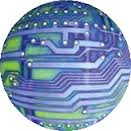
\includegraphics[width=2cm,height=2cm]{elo.jpg}}
\end{picture}
\\
\\
\begin{center}
\textbf{{\LARGE Universidad Técnica Federico Santa María}\\[0.5cm]
{\LARGE Departamento de Electrónica}}\\[4.25cm]
{\Large Informe de Práctica}\\[2.3cm]
{\LARGE \textbf{Centro Cient\'ifico Tecnol\'ogico de Valpara\'iso}}\\[3.5cm]
{\large Arturo Veras Olivos}\\[2cm]
Valparaiso - \today
\\
 {\large Versión 2.5}
\end{center}

%\newpage
%\tableofcontents
%\listoffigures % to produce list of figures
%\listoftables % to produce list of tables
%\newpage
\section*{Informe Semanal de Actividades Realizadas}
\begin{center}

\begin{tabular}{|r|l|}
\hline 
Nombre:  & Arturo Veras\\ 
\hline 
Supervisor & Claudio Torres \\ 
\hline 
Empresa: & CCTVAL \\ 
\hline 
Tipo de Práctica: & Profesional \\ 
\hline 
\end{tabular} 

\end{center}
\subsection*{Semana 1, del \textit{13/01/14 al 17/01/14}}

El trabajo principal se centra en conectar una GPU (Graphic Card Unit) a una
Raspberry Pi (le llamaremos RPi desde ahora), específicamente se quiere
conectar una GT640 la cual tiene una interfaz PCIe 3.0 16x. Cabe destacar que
usar una Rpi no es primordial, es posible que dentro de la investigación se
encuentre una tarjeta que funcione mejor.  La RPi tiene dos interfaces que
estan disponibles para la conexión: (1) el puerto GPIO (General-Purpose
Input/Output) y (2) el puerto USB 2.0 los cuales tendremos que investigar si
sirven para nuestro propósito.  Para realizar la conexión se plantearon las
siguientes ideas:

Se propuso utilizar la tarjeta de desarrollo startKIT, esta tarjeta
particularmente posee una interfaz PCIe  1x la cual podemos utilizar.  Se
propone esta idea porque la tarjeta startKIT se conecta fácilmente a la Rpi a
travs del puerto GPIO.  Esta idea fue descartada porque los drivers de la
interfaz PCIe solo existen para las sliceCARD, estas son tarjetas diseñas
(WIFI, audio, etc.) especialmente para la startKIT. Para conectar la GPU
debemos desarrollar nuestro propio controlador, el que no podemos realizar
debido al limitado tiempo del proyecto.  

La otra idea que surgió fue la de estudiar los adaptadores de PCIe a USB. Estos
utilizan un chip para realizar la tarea el cual, eventualmente, podríamos
utilizar y diseñar una placa para que cumpla nuestros requerimientos, es decir,
conectar la tarjeta PCIe 16x al puerto USB 2.0. Se encontró el chip MCS9901-CC
que es el encargado de realizar el puente entre estas interfaces.  

Una tercera idea es usar un adaptador PCIe a mPCIe llamado PE4L-PM060.  La idea
tras este adaptador es utilizarlo en caso de que se utilice una alternativa a
la Rpi que tenga un puerto mPCIe lo cual es más facil de encontrar en el
mercado.  Esta alternativa tambin fue descartada porque no cumple los
requerimientos. Se encontró un dispositivo que potencialmente puede realizar lo
que necesitamos. 

\subsection*{Semana 2, del 20/01/14 al 24/01/14}

Las tareas de esta semana consisten en seguir buscando otras alternativas ya que las
anteriores han sido descartas por el momento.

Investigando se encontró el dispositivo \textbf{USB2380}. USB2380 un controlador
PCIe 1.0 a USB 2.0. El problema es que para nuestro propósito se necesitará
desarrollar nuestro controlador. Por el momento creemos que esta solución esta
fuera de los objetivos principales, es más, aún no se posee información más
detallada sobre el desarrollo de dicha tarjeta. Otro problema que es que no
sabemos si podemos adquirir el dispositivo a tiempo para realizar pruebas.

Como no se ha encontrado un adaptador directo entre PCIe y USB se decide por
estudiar la posibilidad de realizar una tarjeta que tenga ambas interfaces y que
cumpla con nuestros requerimientos. Las posibilidades son : \textbf{MCS990} PCIe
to 4-Port USB 2.0 Host Controller y \textbf{USB2380} PCIe 1.0 to USB 2.0
controller.

Sin embargo en cualquier caso la conexión de cualquiera de estos dos dispositivos
se realiza a través slot PCIe 1x. La GT640 tiene una interfaz PCIe 16x, esto no
produce ningún problema ya que el protocolo PCIe, en este caso, se adapta al slot
1x disminuyendo el ancho de banda.

Se descarto completamente la posibilidad de usar el chip \textbf{MCS9990} porque
no cumple con los requerimientos.

Otra alternativa que se encontro es el \textbf{SBC-A510 Single Board Computer}. Lo
importante de esta tarjeta es que tiene un puerto mPCIe que podemos utilizar junto
al adaptador \textbf{PE4L-PM060A}. Esta idea la dejamos en stand by.

Por el momento no se puede conectar la RPi a una tarjeta PCIe. La nueva estrategia
será encontrar formas de dejar la tarjeta gráfica como un periférico que pueda
accederse desde un puerto USB asi como dispositvo plug and play.

\subsection*{Semana 3, del 27/01/14 al 31/01/14}

Una de las nuevas estrategias es utilizar una placa madre que tenga un puerto
PCIe. La idea es usar un hardware de bajo consto con los requerimientos mínimos
para que la GT640 funcione. Para esto existen alternativas como placas madres
Micro-ATX, Mini-ITX, Nano-ITX y Pico-ITX, claro está que a medido que la placa
es más pequeña más costosa será. 

Además, insvestigando hemos encontrado una solución muy parecida a lo que
queremos, se trata de una tarjeta desarrollo de llamada Kayla, básicamente es
un computador pequeño que reune todas las características para trabajar con la
tarjeta GT640.  

Se encontro otro dispositivo que en primera instancia cumple con nuestros
requerimientos. La \textbf{USB3380EVB} es una tarjeta de desarrollo que tiene la
version USB 3.0 del \textbf{USB2380} chip previamente mencionado. Esta tarjeta
posee un slot PCIe 1x. Envíamos correos preguntando la factibilidad de nuestro
proyecto.

Se encontro otra tarjeta de desarrollo, el \textbf{86 Duino plataform} la cual
posee el puerto mPCIe el cual podemos utilizar con el adaptador
\textbf{PE4L-PM060A}.

Hasta el momento tenemos las alternativas mencionada, realizamos el presupuesto y
estamos a la espera de la desición.

La alternativa más factible es comprar la \textbf{USB3380EV} y desarrollar el
software necesario para nuestra aplicación. El problema es que el distribuidor
esta de vacaciones por lo que tenemos que esperar hasta la próxima semana.

Mientras estudiamos la posibilidad de utilizar un computador de bajo costo como
interfaz entre la GPU y cualquier host. La conexión sería a trav\'es del USB de
forma plg and play.

La idea de conectar una RPi a la GPU se descarto completamente ya que la RPi no 
tiene la arquitectura necesaria para que CUDA, el software de desarrollo de las GPU de Nvidia, funcione.

\subsection*{Semana 4, del 03/02/14 al 06/02/14}

Esta semana se realizó una revisión de todas las ideas que estaban en el
tapete. Nos dimos cuenta que estabamos dando vueltas y era necesario tener una
nueva estrategia para resolver el problema. Decidimos volver a comenzar de
nuevo, ya con las demás ideas descartadas. Ya que aún no hemos tenido
respuestas satisfactorias sobre el controlador del USB3380 EVK, hemos decidido
construir un computador barato que cumpla con los requerimientos para instalar
la GT640 y CUDA. La idea sobre esto es tener un dispositivo portatil plug and
play, para esto estudiaremos la posibilidad de realizar a traves del puerto usb
o del ethernet. 

Por otro lado en caso de que compremos la tarjeta USB3380 EVK y el desarrollo
del driver sea ráido, hemos buscado computadores de bajo costo para realizar un
cluster. Hemos encontrado el ODROID. Es un computador muy barato para las
grandes características que posee, es compatublible con el driver NVidia y
CUDA.

\subsection*{Semana 5, del 10/02/14 al 14/02/14}
\begin{comment}
lunes
-
Ademas se realizó un estudio sobre como conectar el comptuador de una forma
plug and play, las opciones son utilizar el puerto Ethernet o, mejor aún,
realizar la conexión a trav\'es USB.

martes 
- Reunion con el profesor para ver el estado del proyecto. 3 ideas
  nuevas aparecieron.

miercoles 
- Contacto con un desarrollador de USB3380 para solicitar ayuda en el
  campo. 
- Estudio de RNDIS para conectar usb a usb, existe la posibilidad.

jueves 
- Estudio del funcionamiento de usb. Aprendi que podemos utilizar el
  computador como gadget y realizar la configuración recompilando el kernel y
  agregando los drivers.Mas detalles leer Linux Gadget Drivers
- Aún falta el cable. 
- Compilación del kernel para agregar los módulos. Estamos a la espera
  del cable USB macho macho.

viernes 
- Update del proyecto al profesor Claudio torres. 
 - compramos cable USB 3.0, estamos a la espera del envío.
\end{comment}
\subsection*{Semana 6, del $17/02/14 al 21/02/14$}

Se compro el computador de bajo costo para realizar las primeras pruebas.
Ademas se realizó un estudio sobre como conectar el comptuador de una forma plug
and play, las opciones son utilizar el puerto Ethernet o, mejor aún, realizar la
conexión a trav\'es USB.

\end{document}

